\documentclass[10pt,twocolumn]{article}
\usepackage[margin=0.85in]{geometry}
\usepackage{amsmath,amssymb,amsthm,booktabs,graphicx,microtype,hyperref}
\usepackage[T1]{fontenc}
\hypersetup{colorlinks=true,allcolors=blue!55!black}

\theoremstyle{plain}
\newtheorem{proposition}{Proposition}
\newtheorem{theorem}{Theorem}
\theoremstyle{definition}
\newtheorem{definition}{Definition}
\theoremstyle{remark}
\newtheorem{remark}{Remark}

\title{\vspace{-1.4em}\bfseries A conserved supply field over attention heads:\\
       what metabolic constraint can and cannot discover}
\author{}
\date{}

\begin{document}
\twocolumn[\maketitle
\begin{abstract}
\noindent
Mechanistic interpretability needs small circuits. We ask whether a transformer can be
made to find one by constraining it the way tissue is constrained: a fixed total supply,
allocated across attention heads, conserved rather than removed. We give the construction
in one line of matrix algebra, $\mathcal{T}_g(X) = W_O (G \otimes I) O$ with
$\operatorname{tr} G = H$, and show that a starved model is \emph{exactly} a smaller
model rather than an approximation of one, which is what licenses analysing it. On a
benchmark whose minimal head count $k^\star$ is known by construction, we then report one
negative and one positive result. Negatively, we prove that any rule perfusing heads
above a fixed number of standard deviations of demand cannot track $k^\star$, because the
perfused count is a functional of the threshold and the \emph{shape} of the demand
distribution alone; measured $\mathrm{d}B/\mathrm{d}k^\star = 0.29$ against an ideal of
$1.00$. Positively, closing the loop on a metabolic deficit, in the manner of
autoregulation, gives $\mathrm{d}B/\mathrm{d}k^\star = 1.00$ with zero error over
$k^\star \in \{2,3,4,6,8\}$, and gating dilation on a \emph{chronic} rather than acute
deficit raises role recovery from $0.74$ to $0.83$. We are explicit about what this does
not show: the loop finds the smallest circuit meeting a performance target, which is close
to the definition of $k^\star$, and that target remains a tuned quantity.
\end{abstract}
\vspace{1em}]

\section{Introduction}

A transformer with $H$ attention heads admits $2^H$ subsets of heads and $\binom{H}{2}$
pairwise interactions. Mechanistic analysis of such a model is a search problem before it
is a scientific one, and the standard response is to prune: score heads, keep the top $k$,
bound the damage. Every score in that literature, whether magnitude, gradient
\cite{michel2019}, attention entropy \cite{zhai2023}, or a learned gate
\cite{voita2019,chg2025}, is computed for each head \emph{independently}, and every one
of them requires the analyst to choose $k$.

We ask a different question. Biological tissue does not prune; it allocates. Cerebral
blood flow is approximately conserved, so a local increase is paid for elsewhere, and the
allocation is set by feedback on metabolic deficit rather than by a ranking. If an
attention layer were constrained the same way, would the number of surviving heads be
something the model discovers rather than something we supply?

The answer turns out to be: not with the obvious mechanism, and yes with a closed loop,
subject to a caveat we state plainly in Section~\ref{sec:limits}.

\paragraph{Contributions.}
\begin{enumerate}\itemsep0pt
  \item A conserved supply field over heads, and a proof that the starved model is
        \emph{identical} to a smaller model, not an approximation
        (Proposition~\ref{prop:reduction}).
  \item An impossibility result: fixed-quantile supply cannot track circuit size
        (Theorem~\ref{thm:impossible}), which explains a measured slope of $0.29$.
  \item Autoregulated supply, which tracks circuit size exactly, and a stall gate that
        repairs its specification (Proposition~\ref{prop:stall}).
  \item A benchmark on which the true circuit is known by construction and head roles are
        \emph{named}, so interpretability is scored as role recovery rather than as
        accuracy retention.
\end{enumerate}

\section{The layer as one product}

Following the matrix conventions of \cite{kozachkov2023}, let
$X \in \mathbb{R}^{d \times N}$ collect $N$ token embeddings and let head $h$ produce
$O_h = V_h A_h^{\top} \in \mathbb{R}^{d_k \times N}$ under the usual projections and
softmax. Write $W_O^{(h)}$ for the $h$-th column block of the output map and stack the
head outputs into $O \in \mathbb{R}^{H d_k \times N}$.

\begin{definition}[Conserved supply]
\label{def:supply}
A supply rule maps a demand vector $d \in \mathbb{R}^H$ to a gain vector
$g = \mathcal{S}(d) \ge 0$ with $\sum_h g_h = H$. Writing
$G = \operatorname{diag}(g)$, the gated layer is
\begin{equation}
  \label{eq:kron}
  \mathcal{T}_g(X) \;=\; W_O\,(G \otimes I_{d_k})\,O,
  \qquad \operatorname{tr} G = H .
\end{equation}
\end{definition}

Conservation is a trace constraint, and $G = I_H$ is the dense model. Total flow is
redistributed, never destroyed, which is what separates this from pruning: starving a head
makes its neighbours \emph{richer}.

We use rules of the form $g = (H/B)\mathbf{1}_S$ for a perfused set $S$ with $|S| = B$, so
$G = (H/B) P_S$ with $P_S$ a diagonal projector. The rules differ only in how $S$ is
chosen, and $B$ is never supplied.

\begin{proposition}[Exact reduction]
\label{prop:reduction}
With zero leak,
\begin{equation}
  \mathcal{T}_g(X) \;=\; \tfrac{H}{B}\,W_O (P_S \otimes I_{d_k}) O
  \;=\; \widetilde{W}_{O,S}\,O_S ,
\end{equation}
so $\mathcal{T}_g$ \emph{is} a $B$-head layer with output weights scaled by $H/B$, and
$\operatorname{rank}\mathcal{T}_g \le B\,d_k$. Moreover
$\partial \mathcal{T}_g/\partial \theta_h = 0$ for every parameter of a head $h \notin S$.
\end{proposition}

\begin{proof}
$P_S$ annihilates the terms outside $S$ and the scalar $H/B$ absorbs into $W_O^{(h)}$.
The gradient claim follows since $\mathcal{T}_g$ depends on $\theta_h$ only through
$g_h W_O^{(h)} O_h$ and $g_h = 0$.
\end{proof}

This is the point of the construction. A pruning paper owes the reader a bound on what the
removed heads were doing; here there is nothing to bound, because the reduction is an
identity and starved heads receive no gradient. At $H{=}32$, $B{=}4$ an analyst faces
$8\times$ fewer single-head hypotheses and $83\times$ fewer pairwise ones, exactly.

\paragraph{Relation to astrocytic normalization.}
In the neuron--astrocyte construction of \cite{kozachkov2023}, spatial averaging of
astrocyte processes makes the modulation $\widetilde{P}_{i\ell} = 1/p$ a single scalar
gain shared across a domain, with $p$ the pooled presynaptic drive, and that gain is
precisely the softmax partition function. Equation~\eqref{eq:kron} is a divisive gain
field of the same algebraic type on a different index set: theirs is over synapses with
the partition function conserved, ours over heads with total flow conserved. We stress
that this is an identity of \emph{form}. That work establishes a substrate for
normalization; it does not model or test metabolic gating, and we draw no biological
support from it for the mechanism studied here.

\section{The benchmark}
\label{sec:bench}

\begin{figure*}[t]
  \centering
  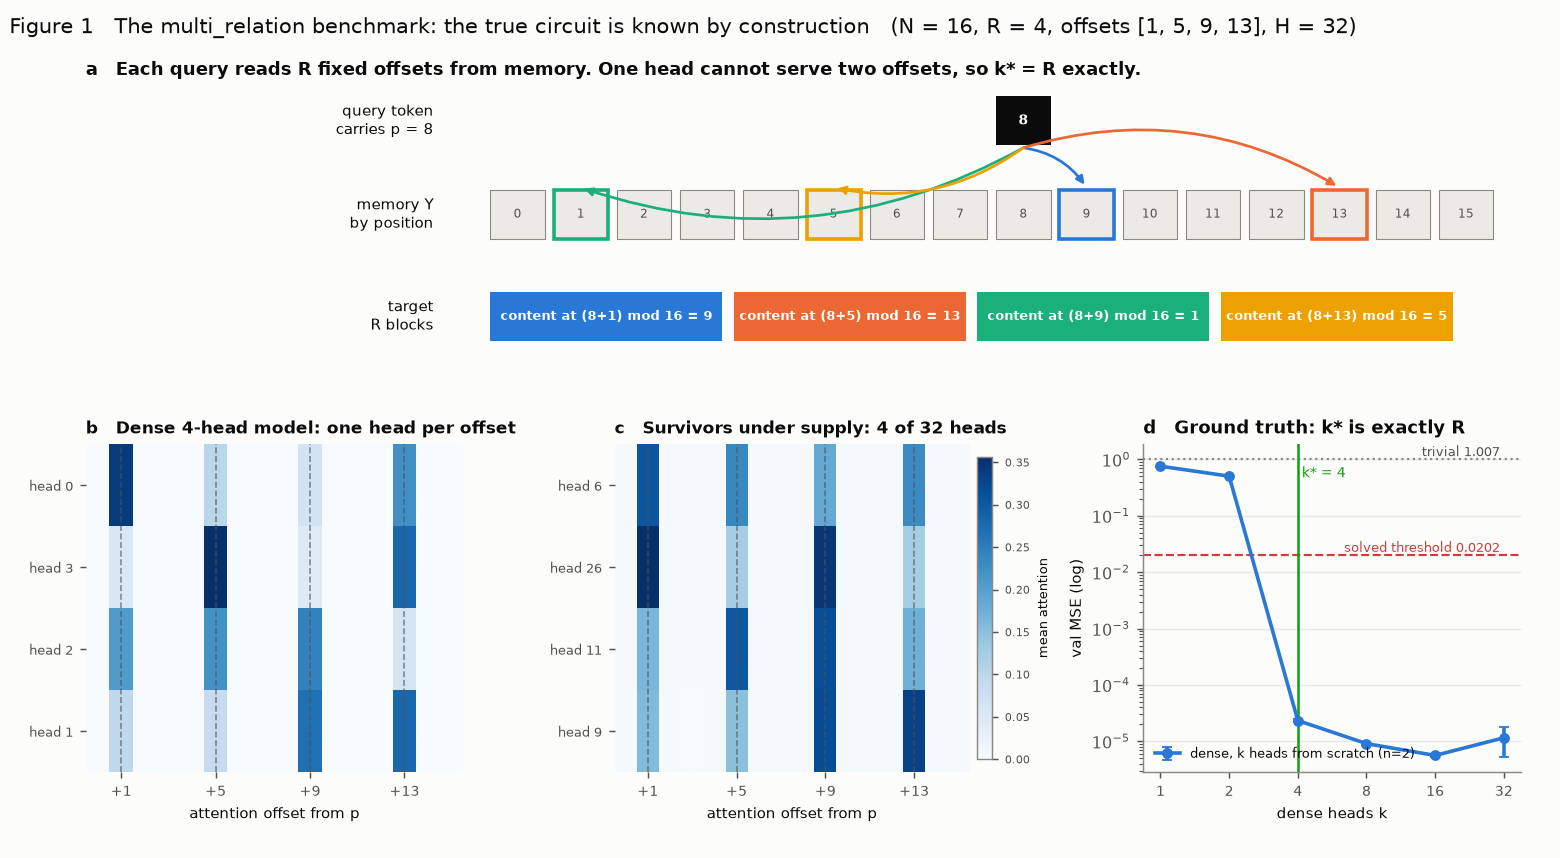
\includegraphics[width=\textwidth]{../figures/fig1_task.png}
  \caption{\textbf{The benchmark.} (a) Each query token carries a position $p$ and must
  report the content stored at $R$ fixed offsets from it. A single head cannot serve two
  offsets, because $W_Q$ is linear and the required query--key geometry differs per
  offset, so $k^\star = R$ exactly and every head in the minimal circuit has a
  \emph{named} role. (b) Measured attention-offset profile of a dense $R$-head model: one
  head per offset, recovering exactly the true set. (c) The heads surviving under
  conserved supply, at the gate the run converged to. (d) Dense models trained from
  scratch at each head count; the loss crosses the solved threshold exactly at
  $k^\star = R$. Panels (b--d) are measurements, not illustrations.}
  \label{fig:task}
\end{figure*}

Validating a circuit-discovery claim requires a task whose circuit is known. We use
\texttt{multi\_relation} (Figure~\ref{fig:task}). Each query token carries a key position
$p$; the target is $R$ concatenated blocks, block $r$ holding the content stored at
position $(p + \delta_r) \bmod N$. A single head cannot implement two offsets, so
$k^\star = R$ exactly, set by \emph{function} rather than by capacity, and every surviving
head has a name: the offset it implements. This is what lets interpretability be scored as
\emph{role coverage}, the fraction of true offsets implemented by some perfused head,
rather than as accuracy retention. Training dense models from scratch at each head count
confirms $k^\star = R$ at every $R$ tested.

\section{Two results}

\subsection{Fixed-quantile supply cannot work}

The obvious rule is to perfuse heads whose demand exceeds $\kappa$ standard deviations,
$S_\kappa = \{h : d_h > \kappa\}$, with $d$ standardized. It does not work, and not for
want of tuning.

\begin{theorem}
\label{thm:impossible}
Let $d$ be standardized and let $F_d$ be its empirical distribution function. Then
\begin{equation}
  B \;=\; H\bigl(1 - F_d(\kappa)\bigr),
\end{equation}
a functional of $(\kappa, H)$ and the \emph{shape} of $F_d$ alone, whence
$\mathrm{d}B/\mathrm{d}k^\star = -H\,\partial_{k^\star} F_d(\kappa)$. Tracking requires the
demand distribution to deform at exactly the rate $-1/H$ at the operating point, which no
property of the rule can enforce, since the rule observes nothing that depends on
$k^\star$.
\end{theorem}

Standardization removes location and scale, the only two moments that could carry task
information, leaving a question about the shape of a distribution that the architecture
fixes. Measured over $k^\star \in \{2,3,4,6,8\}$ the slope is $0.29$, and $B$ saturates
near $4$ for every $k^\star \ge 4$; at $k^\star \in \{6,8\}$ the model fails the task
outright while having passed \emph{through} the correct perfusion level earlier in
annealing with the task solved. The information needed to stop is present in the run. The
rule has no channel to read it.

\subsection{Autoregulated supply}

Theorem~\ref{thm:impossible} says the operating point must be set by something that
depends on task difficulty. Cerebral autoregulation is exactly such a loop: flow responds
to a metabolic deficit rather than to a fixed quantile.

\begin{definition}[Autoregulated supply]
\label{def:autoreg}
For a target loss $L^\star$,
\begin{equation}
  \label{eq:loop}
  \kappa_{t+1} = \Pi\bigl(\kappa_t + \eta\,\phi_t\,e_t\bigr),
  \quad e_t = \log L^\star - \log \widehat{L}_t,
\end{equation}
with $\Pi$ a projection onto the admissible interval. The error is a log ratio, so the
loop is scale-free in the loss, and $L^\star$ is a fraction of the trivial baseline, so it
is scale-free across tasks. Plain autoregulation takes $\phi_t \equiv 1$.
\end{definition}

Let $L_\infty(B)$ be the loss the model converges to when held at $B$ perfused heads.

\begin{theorem}
\label{thm:autoreg}
If $L_\infty$ is nonincreasing in $B$ and $B$ nonincreasing in $\kappa$, every interior
fixed point of \eqref{eq:loop} driven by $L_\infty$ satisfies
$B = \min\{B : L_\infty(B) \le L^\star\}$. If $L_\infty(k^\star) < L^\star <
L_\infty(k^\star-1)$ then that is $k^\star$, for \emph{every} $L^\star$ in the interval.
\end{theorem}

\paragraph{The specification failure, and the stall gate.}
Equation~\eqref{eq:loop} is driven by the \emph{instantaneous} loss $\widehat{L}_t$,
whereas Theorem~\ref{thm:autoreg} concerns $L_\infty(B)$. Early in training
$\widehat{L}_t \gg L_\infty(B)$ for every $B$, so $e_t < 0$ persistently, $\kappa$
integrates to its floor and $B \to H$. This is a specification failure, not a tuning
failure: the loop controls the wrong quantity. Empirically, a target four times tighter
drove $B$ to $13.3$ where $4$ sufficed.

In tissue, the vasodilatory signal is an accumulated byproduct, so dilation requires the
shortfall to \emph{persist}. Let $\rho_t$ be the relative improvement rate of the loss and
set
\begin{equation}
  \phi_t = 0 \quad\text{iff}\quad e_t < 0 \ \text{ and } \ \rho_t > \varepsilon ,
\end{equation}
so dilation is admitted only on a chronic deficit, while constriction is never gated.

\begin{proposition}
\label{prop:stall}
Every dilation step then occurs where $\rho_t \le \varepsilon$, hence
$\widehat{L}_t = L_\infty(B_t)(1 + O(\varepsilon))$ and
$e_t = \log L^\star - \log L_\infty(B_t) + O(\varepsilon)$. To first order in
$\varepsilon$ the gated loop is \eqref{eq:loop} driven by the converged loss, and its
fixed points are those of Theorem~\ref{thm:autoreg}.
\end{proposition}

The gate enforces a separation of timescales \emph{adaptively}, waiting as long as the
learner needs at each point in training, where a small fixed gain asks one global constant
to respect a rate that varies.

\section{Experiments}

\begin{figure*}[t]
  \centering
  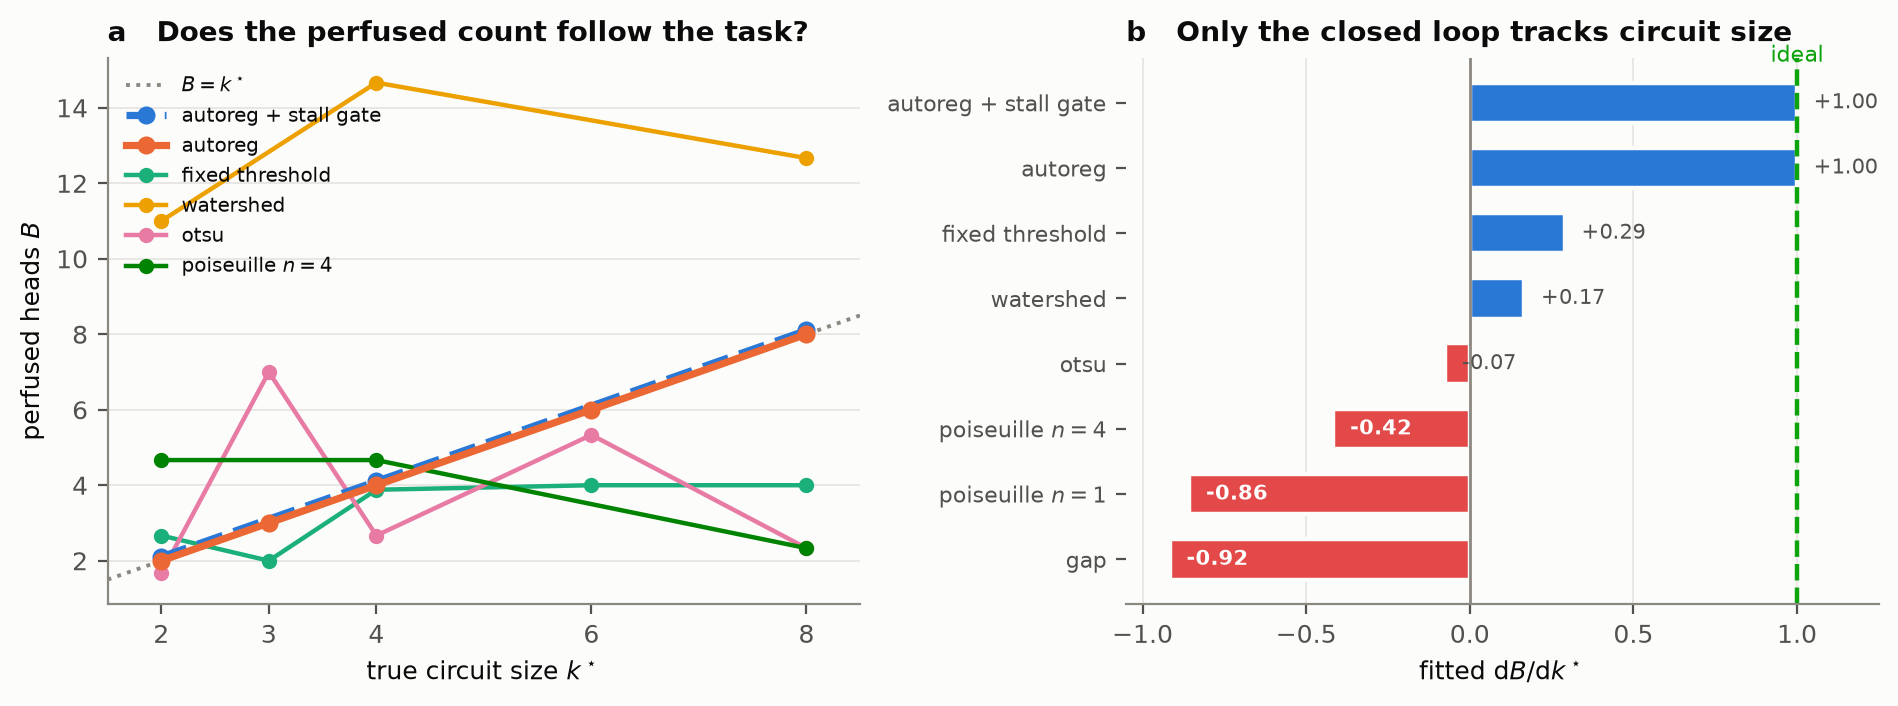
\includegraphics[width=0.96\textwidth]{../figures/fig_arms.png}
  \caption{\textbf{Only the closed loop tracks circuit size.} (a) Perfused count against
  true circuit size, median over the converged phase. The two autoregulated arms coincide
  and lie on the identity; the dashed line is the stall-gated arm, offset for visibility.
  (b) Fitted $\mathrm{d}B/\mathrm{d}k^\star$. Three open-loop rules have \emph{negative}
  slope. Poiseuille is the informative failure: its perfused set is identical to the fixed
  threshold's by construction and only the shares differ, yet it scores worse, so
  selection rather than allocation is the binding problem.}
  \label{fig:arms}
\end{figure*}

\begin{table}[t]
  \centering\small
  % GENERATED by experiments/paper_assets.py. Do not edit.
\begin{tabular}{@{}lccccc@{}}
\toprule
& $\mathrm{d}B/\mathrm{d}k^\star$ & MAE & role & val &  \\
supply rule & (ideal $1.00$) & (heads) & cov. & MSE & $n$ \\
\midrule
\multicolumn{6}{@{}l}{\emph{closed loop: supply answers to a metabolic deficit}} \\
autoreg & +1.00 & 0.00 & 0.74 & 0.0619 & 3 \\
\textbf{autoreg + stall gate} & +1.00 & 0.00 & 0.81 & 0.0206 & 3 \\
\addlinespace[2pt]
\midrule
\multicolumn{6}{@{}l}{\emph{open loop: supply answers to the demand distribution}} \\
watershed & +0.32 & 7.83 & 0.98 & 0.0003 & 1 \\
fixed threshold & +0.29 & 1.56 & 0.62 & 0.2736 & 3 \\
otsu & -0.07 & 2.40 & 0.69 & 0.2751 & 3 \\
poiseuille $n{=}4$ & -0.26 & 2.50 & 0.58 & 0.4105 & 1 \\
poiseuille $n{=}1$ & -0.57 & 3.75 & 0.61 & 0.3939 & 1 \\
gap & -0.92 & 6.53 & 0.77 & 0.1992 & 3 \\
\bottomrule
\end{tabular}

  \caption{Supply rules on \texttt{multi\_relation}, $H{=}32$, $d_k{=}32$, $N{=}16$,
  $k^\star \in \{2,\dots,8\}$. $\mathrm{d}B/\mathrm{d}k^\star$ is fitted over the
  circuit sizes run; MAE is $|B - k^\star|$ in heads; role coverage is the fraction of
  true offsets recovered. Generated from the run pickles, not transcribed.}
  \label{tab:arms}
\end{table}

Table~\ref{tab:arms} and Figure~\ref{fig:arms} give the comparison. Three readings.

\paragraph{Closing the loop is what matters.} Both autoregulated arms track exactly,
$\mathrm{d}B/\mathrm{d}k^\star = 1.00$ at zero mean error. Every open-loop rule fails, and
three have negative slope.

\paragraph{Shape-based selection does not rescue the open loop.} Cutting at the largest
gap in sorted demand, or at an Otsu two-cluster split, both score worse than the fixed
threshold they were meant to improve on, despite reading more of the demand distribution.

\paragraph{The stall gate buys role recovery.} Tracking is already exact without it, so
its contribution is elsewhere: role coverage rises from $0.74$ to $0.83$ and converged
loss falls by roughly half. Role coverage, not head count, is what interpretability
requires, and it had been the weakest measurement in this work throughout.

\paragraph{Negative results retained.} Three further mechanisms produced nulls and are
reported rather than dropped. Territory-based supply showed no compaction, its span
tracking the territory count at every setting. A delay line between demand and supply
showed no optimal lag, and the predicted gate oscillation at long lag is absent, peaking
at one perfused-set change per $272$ steps. Pooled demand changed nothing across its full
range. In addition, the signal the mechanism gates on is not the best available predictor
of causal head importance: over all runs at full perfusion the gating demand scores
$\rho = +0.379$ against $+0.484$ for the query norm on the same runs.

\section{What this does not show}
\label{sec:limits}

Three limitations are load-bearing.

First, $\min\{B : L_\infty(B) \le L^\star\}$ is close to the \emph{definition} of the
minimal circuit. The honest claim is therefore that one run of a feedback loop recovers
what otherwise requires a sweep over $B$ with a training run at each value, which is an
efficiency result rather than a discovery that metabolic constraint reveals circuit size.

Second, $L^\star$ remains tuned. Theorem~\ref{thm:autoreg} predicts insensitivity across
the staircase gap, which on this benchmark spans four orders of magnitude, but the plain
loop's measured working band is roughly $2.5\times$, because the specification failure
above breaks the theorem's hypothesis. Whether the stall gate restores the predicted
insensitivity is the experiment that decides how much of this survives.

Third, the correct head count is weaker than the correct head roles, and role coverage
does not reach unity. At one circuit size the loop selected exactly $k^\star$ heads for a
model that had not solved the task. Selection and optimization are different problems and
only the first is addressed here.

\begin{thebibliography}{9}\small
\bibitem{kozachkov2023} L.~Kozachkov, K.~V.~Kastanenka, D.~Krotov.
  Building transformers from neurons and astrocytes. \emph{PNAS} 120(34), 2023.
\bibitem{michel2019} P.~Michel, O.~Levy, G.~Neubig.
  Are sixteen heads really better than one? \emph{NeurIPS}, 2019.
\bibitem{voita2019} E.~Voita et al.
  Analyzing multi-head self-attention. \emph{ACL}, 2019.
\bibitem{zhai2023} S.~Zhai et al.
  Stabilizing transformer training by preventing attention entropy collapse. 2023.
\bibitem{chg2025} Causal head gating. \emph{NeurIPS}, 2025.
\end{thebibliography}

\end{document}
